\chapter{Phasors}
\section{Exponential inputs and outputs}
Phasors are a ubiquitous method for understanding particular responses of linear differential equations, given sinusoidal input.
The following differential equation is familiar as the capacitor voltage of an RC circuit with \(v_\text{in}\) across both components:
\begin{align}
  \dod{}{t} v_\text{o}
  &= -\frac{1}{RC} v_\text{o} + \frac{1}{RC} v_\text{in},
  \quad \lambda = -\frac{1}{RC}
  \intertext{\autoref{eq:RC-cosine-solution} showed the solution to this differential equation with \(v_\text{in} = V_\text{in} \cos \omega t\), purportedly obtained by direct substitution. While that works, an easier way to the solution is to practice on a general exponential input:}
  v_\text{in}
  &= V_\text{in} e^{st}.
  \intertext{Assuming that \(v_\text{o} = V_\text{o}e^{st}\) is also exponential with the same rate \(s\),}
  s V_\text{o} e^{st}
  &= -\frac{1}{RC} V_\text{o} e^{st} + \frac{1}{RC} V_\text{in} e^{st} \\
  V_o &= \frac{1}{1 + sRC} V_\text{in} = \frac{1}{1 - \frac{s}{\lambda}} V_\text{in}
  \intertext{If our circuit has not existed with its input forever, then the  solution for \(v_\text{o}\) is a superposition of \(V_\text{o}e^{st}\) with a homogeneous response, in which \(A\) is a constant that depends on the initial condition.}
  v_\text{o}
  &= V_\text{o} e^{st}
   \underbrace{{} + A e^{\lambda t}}_{\to 0 \ \text{if} \Re{\lambda} <  0}
  \intertext{If \(\lambda\) has a negative real part, then the impact of the initial condition tends to zero as \(t\to \infty\).
  Sinusoidal inputs and outputs arise as superpositions of exponentials where \(s\) has no real part:}
  s &= j\omega \rightsquigarrow e^{st} = \cos \omega t  + j\sin\omega t\\
  \cos \omega t &= \Re{e^{j\omega t}} = \Re{\cos \omega t + j\sin \omega t} \\
  \cos \omega t &= \frac{1}{2} \del{e^{j\omega t} + e^{-j\omega t}}\\
  \sin \omega t &= \frac{1}{2j} \del{e^{j\omega t} - e^{-j\omega t}}
\end{align}

\section{Phasor representation of a sinusoid}
A phasor is a complex number that has amplitude and phase information of a time-domain sinusoid.
By writing the following cosine as the real part of a complex exponential, we can factor the phasor part from the time-varying part.
\begin{align}
  x(t) &= A \cos (\omega t + \phi), \quad A \ \text{real, positive}\\
  &= \Re\sbr{A e^{j\del{\omega t + \phi}}}\\
  &= \Re\sbr{\underbrace{Ae^{j\phi }}_{\text{phasor}}{e^{j\omega t}}}
\end{align}
The phasor representation of \(A \cos (\omega t + \phi)\) is \(Ae^{j\phi }\).
\(\phi\) is the \emph{phase} of this sinusoid.

\subsection{Uniqueness}
Phasors uniquely represent the sinusoids that they represent.
Suppose we assign the phasors \(A_1\) and \(A_2\) to sinusoids \(x_1\) and \(x_2\), respectively:
\begin{align}
    x_1(t) &= \Re{A_1 e^{j\omega t}}
    \xrightarrow{\text{phasor representation}} A_1 \\
    x_2(t) &= \Re{A_2 e^{j\omega t}}
    \xrightarrow{\text{phasor representation}} A_2
\end{align}

Uniqueness means that
\(
  \del{x_1 = x_2} \iff \del{A_1 = A_2}
\).
We can see see that \(A_1 = A_2\) implies \(x_1 = x_2\), because the identity \(\Re{A_1e^{j\omega t}} = \Re{A_2e^{j\omega t}}\) follows immediately from \(A_1 = A_2\).

To show that \(x_1 = x_2\) implies \(A_1 = A_2\), we verify the real and imaginary layers of this equation independently.
The real part emerges at
\(t=0\): \(x_1(0) = \Re\cbr{A_1}\) and
\(x_2(0) = \Re\cbr{A_2}\).
Therefore \(\Re\cbr{A_1} = \Re\cbr{A_2}\).
On the other hand, we need \(t = \frac{\pi}{2} \frac{1}{\omega}\) to access the imaginary part.
From
\begin{align}
  \left.x_1\right|_{t = \frac{\pi}{2} \frac{1}{\omega}}
  &=
  \left.x_2\right|_{t = \frac{\pi}{2} \frac{1}{\omega}}
  \intertext{follows}
  \Re\cbr{A_1 e^{j\frac{\pi}{2}}}
&= \Re\cbr{A_2 e^{j\frac{\pi}{2}}}.
  \intertext{Applying \(e^{j\frac{\pi}{2}} = j\),}
  \Re\del{A_1j} &= \Re\del{A_2j} \\
  \Re\sbr{\Re\del{A_1}j + j^2 \Im\del{A_1}}
&= \Re\sbr{\Re\del{A_1}j + j^2 \Im\del{A_1}} \\
  -\Im\del{A_1} &= -\Im\del{A_2}
\end{align}

\subsection{Linearity}
Linearity of the phasor transformation means that a real linear combination of sinusoids is represented as the same linear combination of the sinusoids' respective phasors.
For real constants \(a_1\) and \(a_2\), the phasor representation of \(a_1 x_1(t) + a_2 x_2(t)\) is \(a_1 A_1 + a_2 A_2\).
Beginning with our two sinusoids as real parts of scaled complex exponentials,
\begin{align}
  x_1(t) &= \Re\del{A_1 e^{j\omega t}} \\
  x_2(t) &= \Re\del{A_2 e^{j\omega t}},
  \intertext{we may form the following linear combination with real coefficients \(a_1\) and \(a_2\):}
  a_1 x_1(t)
+  a_2 x_2(t)
&= \Re\del{a_1 A_1 e^{j\omega t}} +
\Re\del{a_2 A_2 e^{j\omega t}} \\
&= \Re\sbr{\del{a_1 A_1 + a_2 A_2} e^{j\omega t}}.
\end{align}

\subsection{Differentiation}
Phasors represent differentiation in time as multiplication by \(j\omega\):
if
\begin{align}
  x(t) &= \Re\sbr{A e^{j\omega t}}, \\
  \intertext{then}
  \dod{}{t} x(t) &= \Re\sbr{\underbrace{\ j\omega A\ }_{\text{new phasor}} e^{j\omega t}}.
\end{align}

\section{Current and voltage phasors in circuits}
These three properties translate circuit laws from time domain into phasor domain:
\begin{alignat}{6}
&&
&& \text{\em time} &
\quad&& \longleftrightarrow
\quad& \text{\em phasor} & \notag\\
  &&\text{(\scshape kvl)}
  \qquad&& \sum_{\text{loop}} v &= 0
  \quad&& \longleftrightarrow
  \quad& \sum_{\text{loop}} V &= 0 \\
  &&\text{(\scshape kcl)}
  \qquad&& \sum_{\text{node}} i &= 0
  \quad&& \longleftrightarrow
  \quad& \sum_{\text{node}} I &= 0
\intertext{as well as current-voltage relationships:}
&&\text{(resistor)}
\qquad&& v&= Ri
\quad&& \longleftrightarrow
\quad& V &= RI \\
&&\text{(capacitor)}
\qquad&& i &= C\od{}{t} v
\quad&& \longleftrightarrow
\quad& I &= j\omega CV \\
&&\text{(inductor)}
\qquad&& v &= L\od{}{t} i
\quad&& \longleftrightarrow
\quad& V &= j\omega LI
\end{alignat}

\subsection{RC revisited}
\begin{figure}
  \centering
  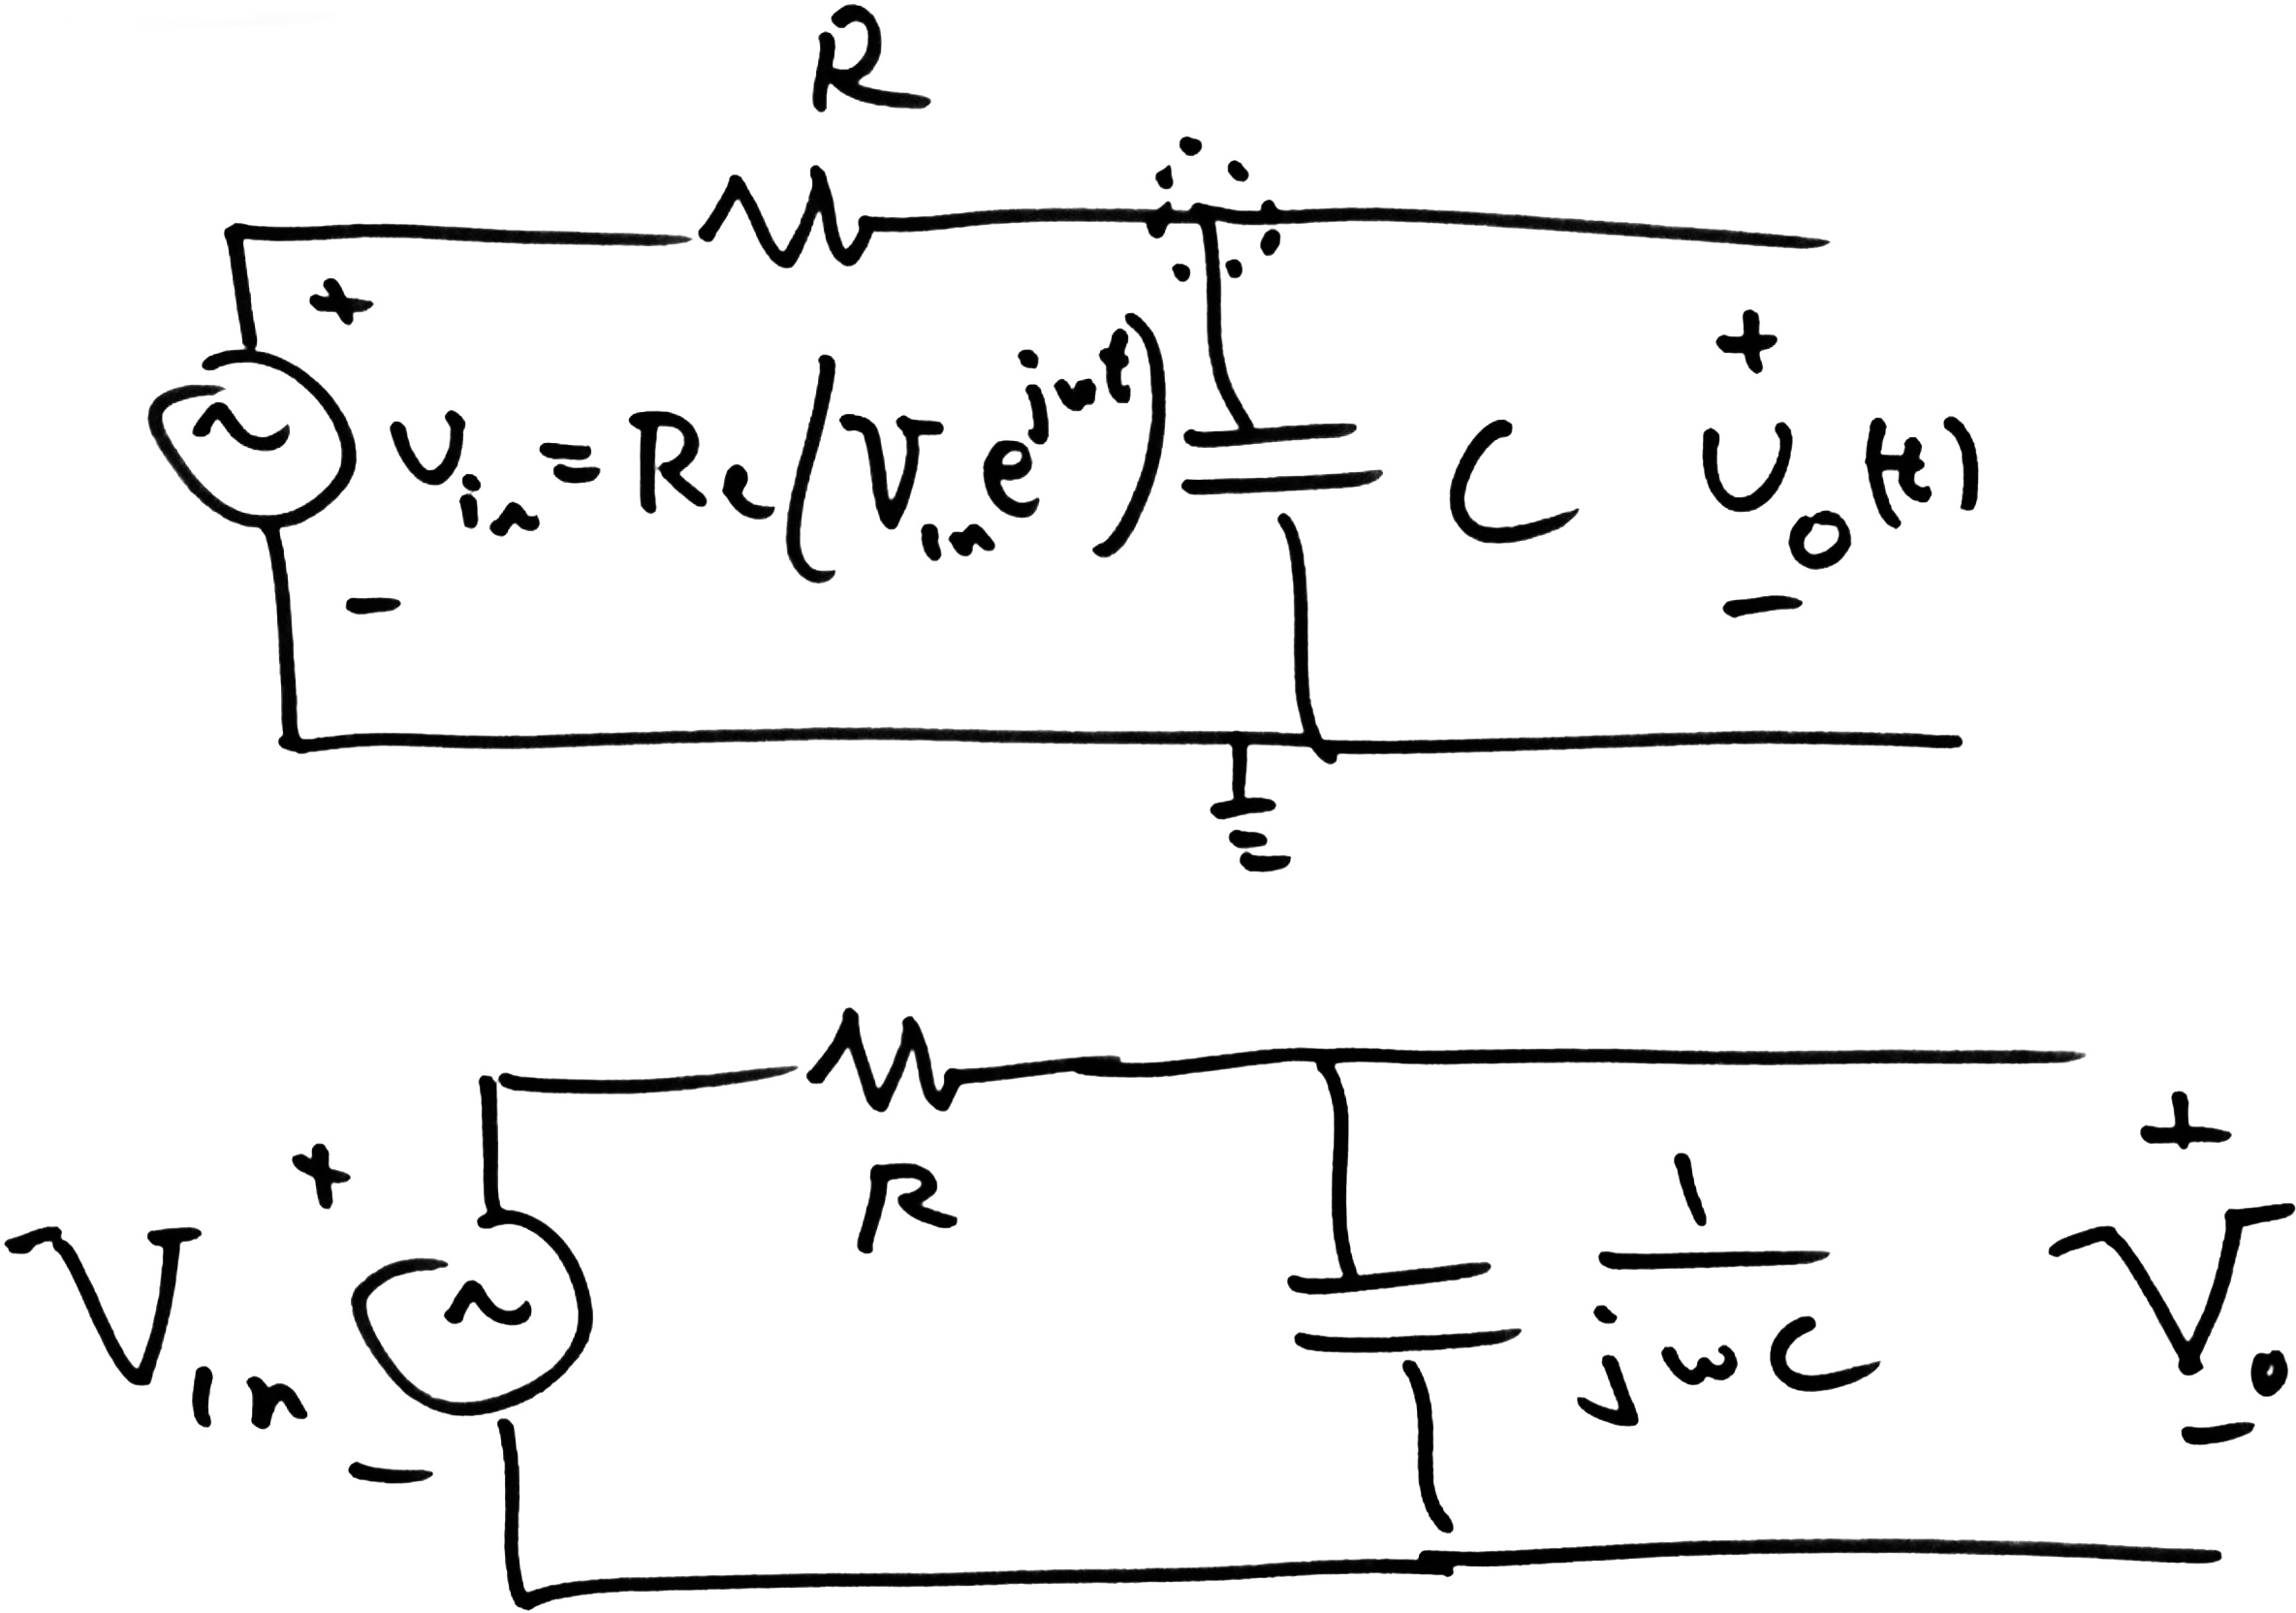
\includegraphics[width=0.5\linewidth]{figures/8/RC-to-phasor}
  \caption{An RC circuit with a sinusoidal voltage source and its phasor domain representation.}
  \label{figure:lec8-RC}
\end{figure}
Because capacitors establish a proportional relationship between their voltage and current phasors, they may be regarded as impedances in phasor domain having impedance \(\frac{1}{j\omega C}\).
A sinusoidally-excited RC circuit is translated into phasor domain in \autoref{figure:lec8-RC}.
In phasor domain, \(V_\text{o}\) is recognized as the lower half of a voltage divider spanning \(V_\text{in}\):
\begin{align}
  V_\text{o} &= \frac{\frac{1}{j\omega C}}{\frac{1}{j\omega C} + R} V_\text{in} \\
  &= \frac{1}{1 + j\omega CR} V_\text{in} \label{eq:lec8-transferfunction}
\intertext{Converting back to time domain,}
v_\text{o}(t)
&= \Re\cbr{V_o e^{j\omega t}} \\
&= \Re\cbr{\frac{1}{1 + j\omega CR} V_\text{in} e^{j\omega t}} \\
\intertext{Changing \(V_\text{o}\) to polar form,}
&= \Re\cbr{\frac{1}{\left|1 + j\omega CR\right| e^{j\angle\del{1 + j\omega CR}}} V_\text{in} e^{j\omega t}} \\
&= \Re\cbr{\frac{1}{\left|1 + j\omega CR\right| e^{j\tan^{-1}\del{\omega CR}}} V_\text{in} e^{j\omega t}} \\
&= \Re\cbr{\frac{V_\text{in}}{\left|1 + j\omega CR\right|} e^{j\del{\omega t - \tan^{-1}\del{\omega CR}}}} \\
v_\text{o}(t)
&= \frac{V_\text{in}}{\left|1 + j\omega CR\right|} \cos{\del{\omega t - \tan^{-1}\del{\omega CR}}}
\end{align}
For low frequencies (\({\omega RC} \ll 1\)), \(\left|V_\text{o}\right| \approx \left|V_\text{in}\right|\).
The output has about the same amplitude as the input.
For high frequencies (\({\omega RC} \ll 1\)),\footnote{The approximation is good when \({\omega RC} > 10\).}
\(\left|V_\text{o}\right| \approx \frac{1}{\omega RC}\left|V_\text{in}\right|\).
As the amplitude at the filter output vanishes at high frequencies, this RC circuit functions as a low-pass filter.
